
\chapter{Colloid diffusion in glass capillary tubes}

\label{extras}

\section{Introduction}
Understanding outliers is the key to describing many important phenomena, including biological processes dependent on the interactions between strands of DNA, patient zero spreading a virus to a new area in a pandemic, many chemical processes, and how microscopic price fluctuations relate to long-term macroscopic trends in the stock market \cite{zhang_first-passage_2016, hufnagel_forecast_2004, redner_8_2001, liu_anchoring_2017}. How do we predict the behavior of these outliers? In diffusive environments, where many particles spread outward from their originating source, we can use Einstein’s theory of diffusion to describe the bulk behavior of the particles \cite{einstein_uber_1905, von_smoluchowski_zur_1906}. Einstein described diffusion as particles undergoing independent random walks. The random-walk description ignores the effect the shared environment has on the particles, resulting in its potential failure to correctly describe the diffusion of the outliers. Particles near each other should be influenced by the medium in the same way, but in Einstein’s theory of diffusion, their behavior is totally independent from one another. As a result, when analyzing the system as a whole, the distributions of outlier particle locations and first passage times will differ from those predicted by Einstein’s theory. The objective of this work is to show this discrepancy experimentally and demonstrate the need for a new theory of extreme diffusion. This is done by studying the first passage times of micron-sized silica beads suspended in water travelling in glass capillary tubes.
 
\section{Background}

\begin{figure}[hb]
\begin{center}
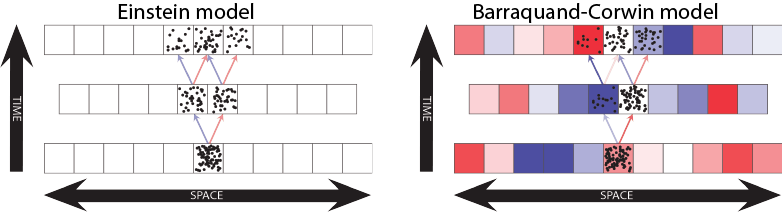
\includegraphics[width=0.9\columnwidth]{Figures/model_both_sidebyside.png}
\caption{\label{fig:1D_BC} 1D visualization of the Einstein and Barraquand-Corwin models, where the red and blue colors indicate the direction of each bias - right and left, respectively - and the color intensity indicates the strength of the bias; for example, a dark red square indicates a strong bias to the right for the particles inhabiting that square. White squares have an equal bias in each direction. Time increases from the bottom of the image toward the top.}
\end{center}
\end{figure}

\begin{figure*}[htp]
\begin{center}
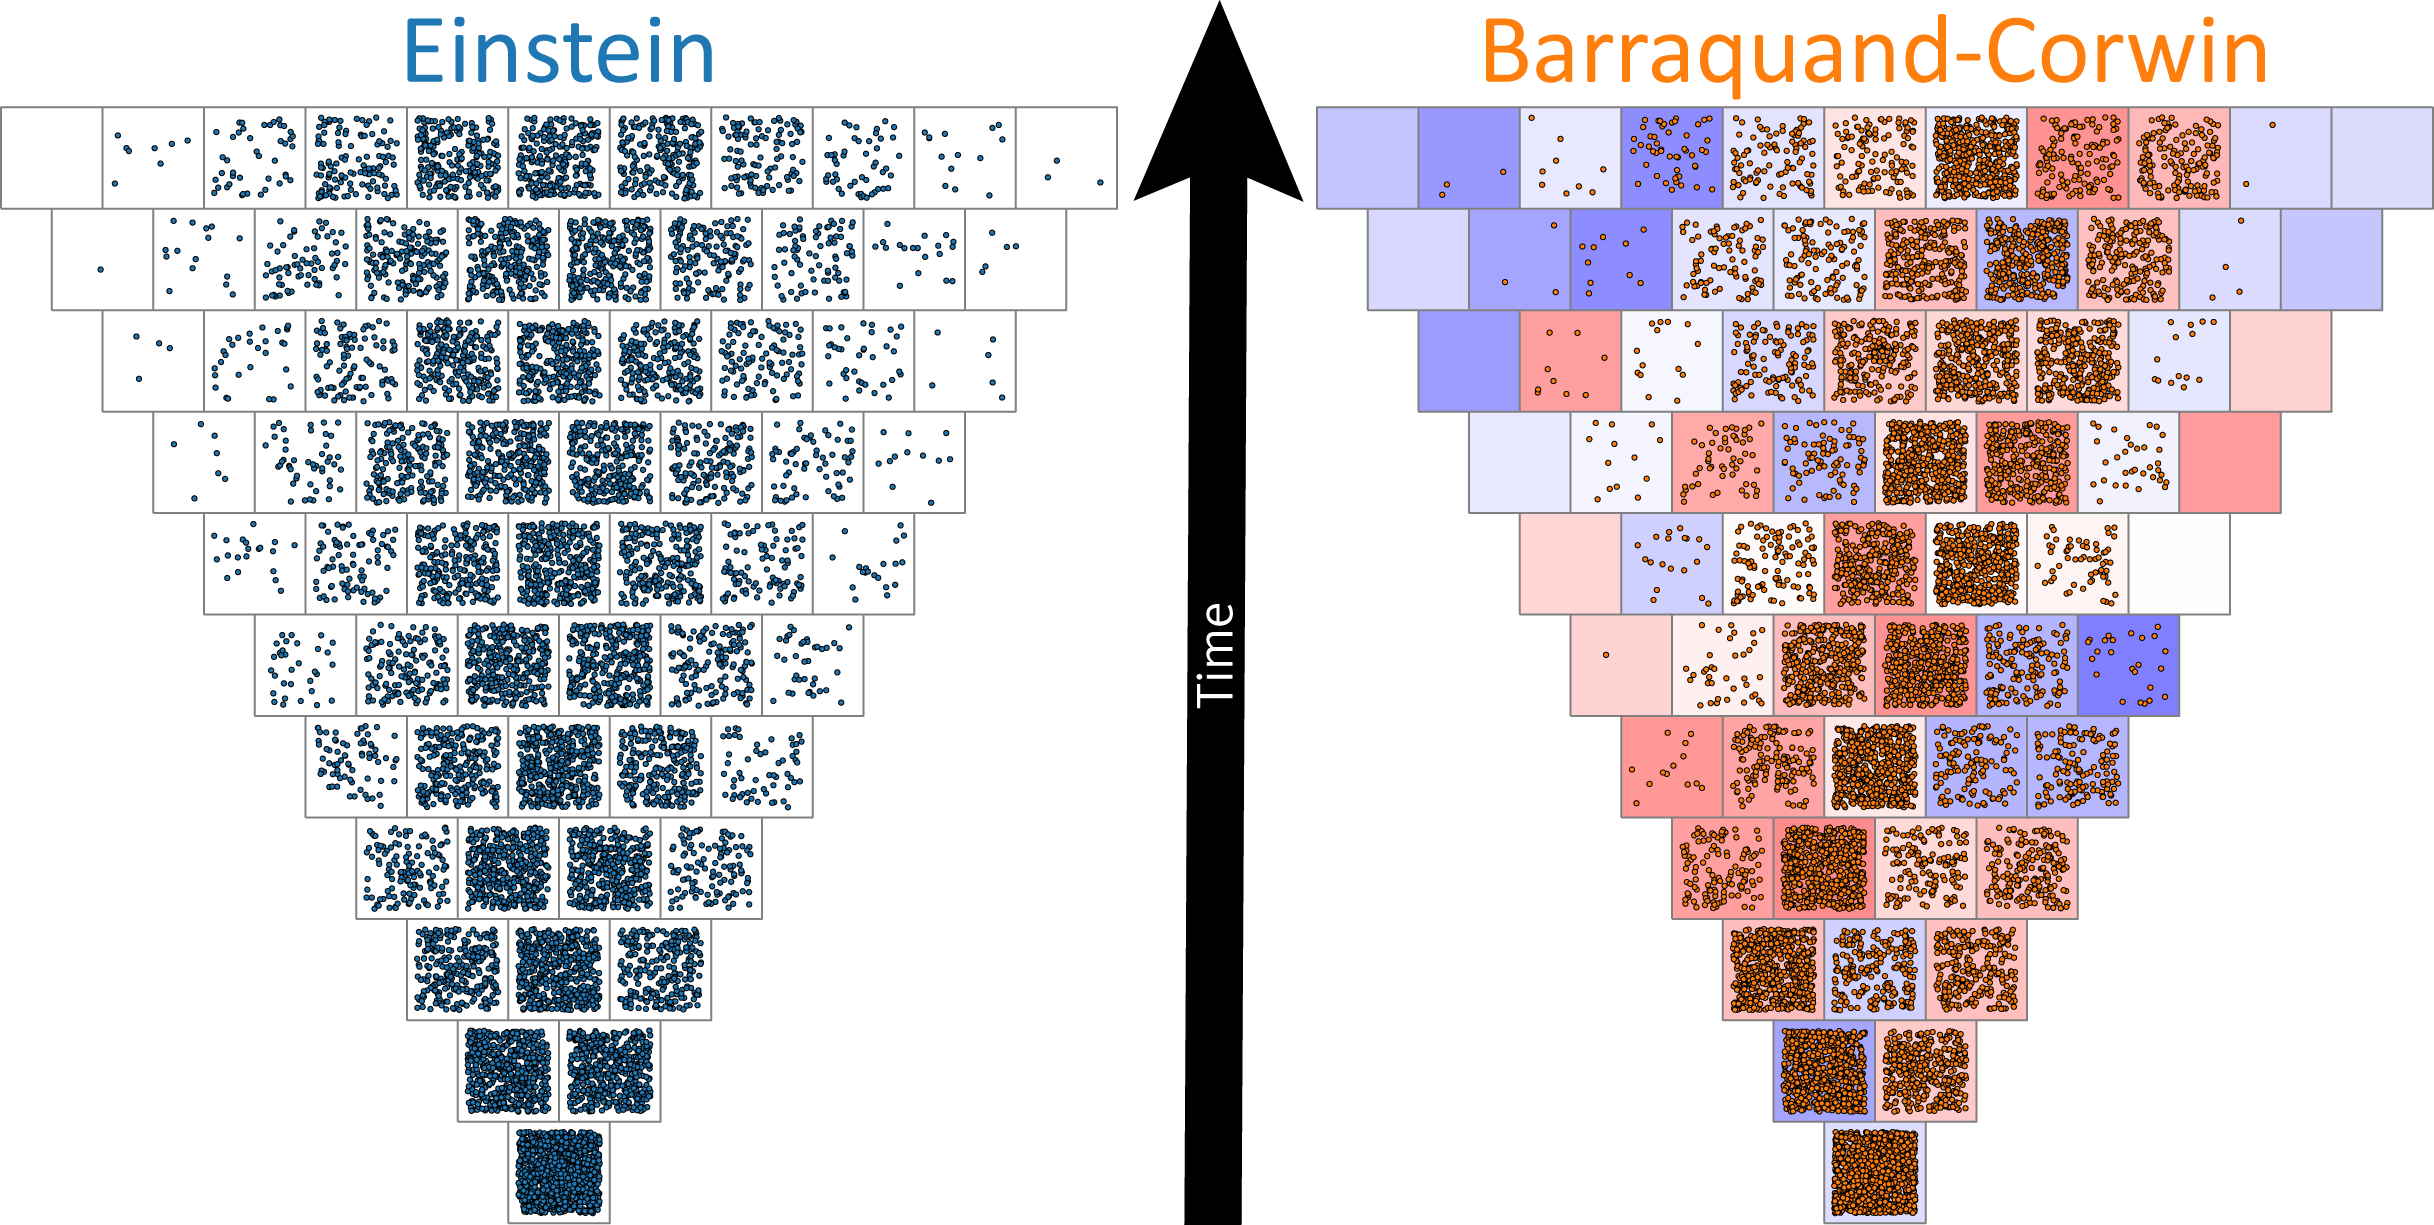
\includegraphics[width=0.9\columnwidth]{Figures/TriangleGrowth-01.png}
\caption{\label{fig:comparison} Einstein and Barraquand-Corwin diffusion models. Einstein's diffusion model has an equal bias in each direction, and the particles diffuse accordingly. For the Barraquand-Corwin model, the red and blue colors and color intensity indicate the direction and strength of the bias as in Figure \ref{fig:1D_BC}. Time increases from the bottom of the image toward the top. There is a noticeable difference in how the outlier particles for each model spread in the same amount of time.}
\end{center}
\end{figure*}

While Einstein's model works for many systems, as scientists have continued to study diffusion, they have discovered areas where this theory and its predictions begin to fail. Some systems, such as Brownian motion in supercooled liquids and close to jamming, flow and drainage, friction, and turbulence, display Brownian motion that lacks a Gaussian distribution\cite{wang_when_2012}. The distributions for such systems instead possess features like exponential tails and other phenomena \cite{metzler_brownian_2019, wang_when_2012}. Additionally, Einstein’s theory fails to accurately capture all the dynamics of active matter where particles inject energy into the environment, like systems with self-propelled particles that display loopy trajectories and non-Gaussian probability distribution function features \cite{kanazawa_loopy_2020, ramaswamy_mechanics_2010}. The nature of these systems introduces correlation, where the energy introduced by the moving particles is shared. The difference between systems with these dynamic particles and those modelled well by independent random walk diffusion is reflected in the statistics describing the system.

It has been assumed that studying extreme diffusion would not lead to anything other than the Einstein model results: each particle moves independently, producing a location distribution with a width related to $t^{\frac{1}{2}}$ and a first passage time distribution that can be categorized as a Lévy distribution. Studying and modelling first-passage particle behavior has been done, but this work has neglected systems where particle motion is correlated \cite{grebenkov_exact_2020}. Recently, Guillaume Barraquand and Ivan Corwin have developed a theoretical model for diffusion that explicitly includes correlations resulting from the shared background environment by modelling diffusion as a random walk with transition probabilities drawn from the beta distribution \cite{barraquand_random-walk_2017}. The beta distribution describes a distribution where the probability distribution function is proportional to $x^{\alpha-1}\left(x-1\right)^{\beta-1}$, and for the Barraquand-Corwin model, $\alpha = \beta$. In the case of a uniform bias, $\alpha = \beta = 1$. Einstein's diffusion model can be considered the case where $\alpha = \beta \rightarrow \infty$. Totally sticky Brownian motion, where all particles move to the right or left together, is the case where $\alpha = \beta \rightarrow 0$.

The Barraquand-Corwin model predicts the behavior of the maximum of a large number of ``walkers’’ and reveals a connection to the Kardar-Parisi-Zhang universality class with a related phase transition \cite{barraquand_random-walk_2017, barraquand_moderate_2020, le_doussal_diffusion_2017, kardar_dynamic_1986}. Figure \ref{fig:1D_BC} shows the Barraquand-Corwin model visually. Figure \ref{fig:comparison} shows the Barraquand-Corwin and Einstein models side-by-side. While bulk diffusion remains the same when going from the Einstein to the Barraquand-Corwin model, the outlier diffusion behaves differently due to the introduced correlation, which is noticeable when comparing the edges of the individual spreads in Figure \ref{fig:comparison} with each other. Hass et. al. characterized extreme diffusion in the random environment model numerically in [cite paper], where the bulk behavior was confirmed to remain the same but a new phase exists for the outlier particles. For the theoretical model that forms the basis of the numerical simulations in this paper, in times comparable to $log\left(N\right)$, there is a connection between the large deviations of transition probabilities in a random walk in random environment (RWRE) and the Kardar-Parisi-Zhang (KPZ) universality class's Tracy-Widom GUE distribution [cite lots of papers, see Hass paper]. In  the $log\left(N\right)^{2}$ time frame, the Tracy-Widom GUE distribution is replaced by that of the KPZ equation [also cite things from Hass paper, and Hass paper]. Numerical simulations confirmed these scalings in these regimes [Hass paper].
%

\begin{figure*}[htp]
\begin{center}
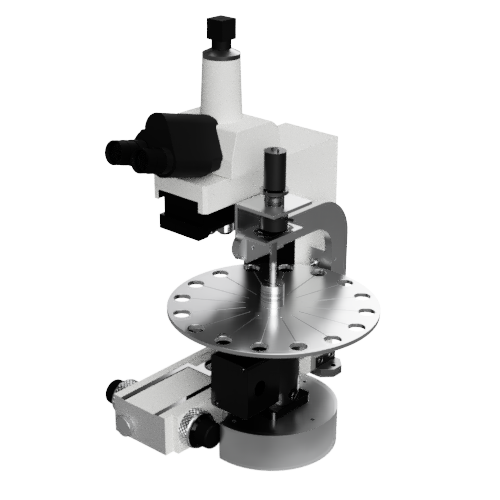
\includegraphics[width=0.9\columnwidth]{Figures/microscope_centrifuge_1.png}
\caption{\label{fig:CADrender} Experimental setup}
\end{center}
\end{figure*}

\section{Experimental design}
To measure EFPTs in a physical system of colloids, I developed a microscope-centirfuge system. Premise:
\begin{itemize}
    \item Colloid suspensions
    \item Capillary tubes (quasi-1D, square for imaging)
    \item Centrifuge servo motor system for spinning down and cycling through for time lapse
    \item Nikon microscope for imaging
    \item Camera for imaging through microscope
    \item Arduino for control through MATLAB
    \item Image analysis via MATLAB? python? can't remember
    \item Bovine whatever serum for coating the glass
    \item whatever was done to minimize air pockets
\end{itemize}
 
\section{Results}
\begin{itemize}
    \item Centrifuge works
    \item Servo positioning works
    \item Time lapse works
    \item Image stabilization, processing
    \item Preliminary tracking
    \item Coating tube minimizes sticking
    \item Removing bubbles
\end{itemize}

\section{Discussion/Conclusion}
\begin{itemize}
    \item Basic process works
    \item More work needs done
    \item Accurate predictions?
    \item Proof of concept essentially
\end{itemize}
%%

%\bibliography{scaling}% Produces the bibliography via BibTeX.


%\end{document}
%
% ****** End of file aipsamp.tex ******

